%%%%%%%%%%%%%%%%%%%%%%%%%%%%%%%%%%%%%%%%%
% baposter Portrait Poster
% LaTeX Template
% Version 1.0 (15/5/13)
%
% Created by:
% Brian Amberg (baposter@brian-amberg.de)
%
% This template has been downloaded from:
% http://www.LaTeXTemplates.com
%
% License:
% CC BY-NC-SA 3.0 (http://creativecommons.org/licenses/by-nc-sa/3.0/)
%
%%%%%%%%%%%%%%%%%%%%%%%%%%%%%%%%%%%%%%%%%

%----------------------------------------------------------------------------------------
%	PACKAGES AND OTHER DOCUMENT CONFIGURATIONS
%----------------------------------------------------------------------------------------

\documentclass[a0paper, portrait]{baposter}

\usepackage[font=small, labelfont=bf]{caption} % Required for specifying captions to tables and figures
\usepackage{booktabs} % Horizontal rules in tables
\usepackage{relsize} % Used for making text smaller in some places
\usepackage{enumitem} % Use for small margin bullet lists
\usepackage{xcolor} % Colour of text
\graphicspath{{figures/}} % Directory in which figures are stored

\definecolor{bordercol}{RGB}{40,40,40} % Border color of content boxes
\definecolor{headercol1}{RGB}{186,215,230} % Background color for the header in the content boxes (left side)
\definecolor{headercol2}{RGB}{80,80,80} % Background color for the header in the content boxes (right side)
\definecolor{headerfontcol}{RGB}{0,0,0} % Text color for the header text in the content boxes
\definecolor{boxcolor}{RGB}{186,215,230} % Background color for the content in the content boxes Use c1d0e1 to rem

\begin{document}

\background{ % Set the background to an image (background.pdf)
\begin{tikzpicture}[remember picture,overlay]
\draw (current page.north west)+(-2em,2em) node[anchor=north west]
{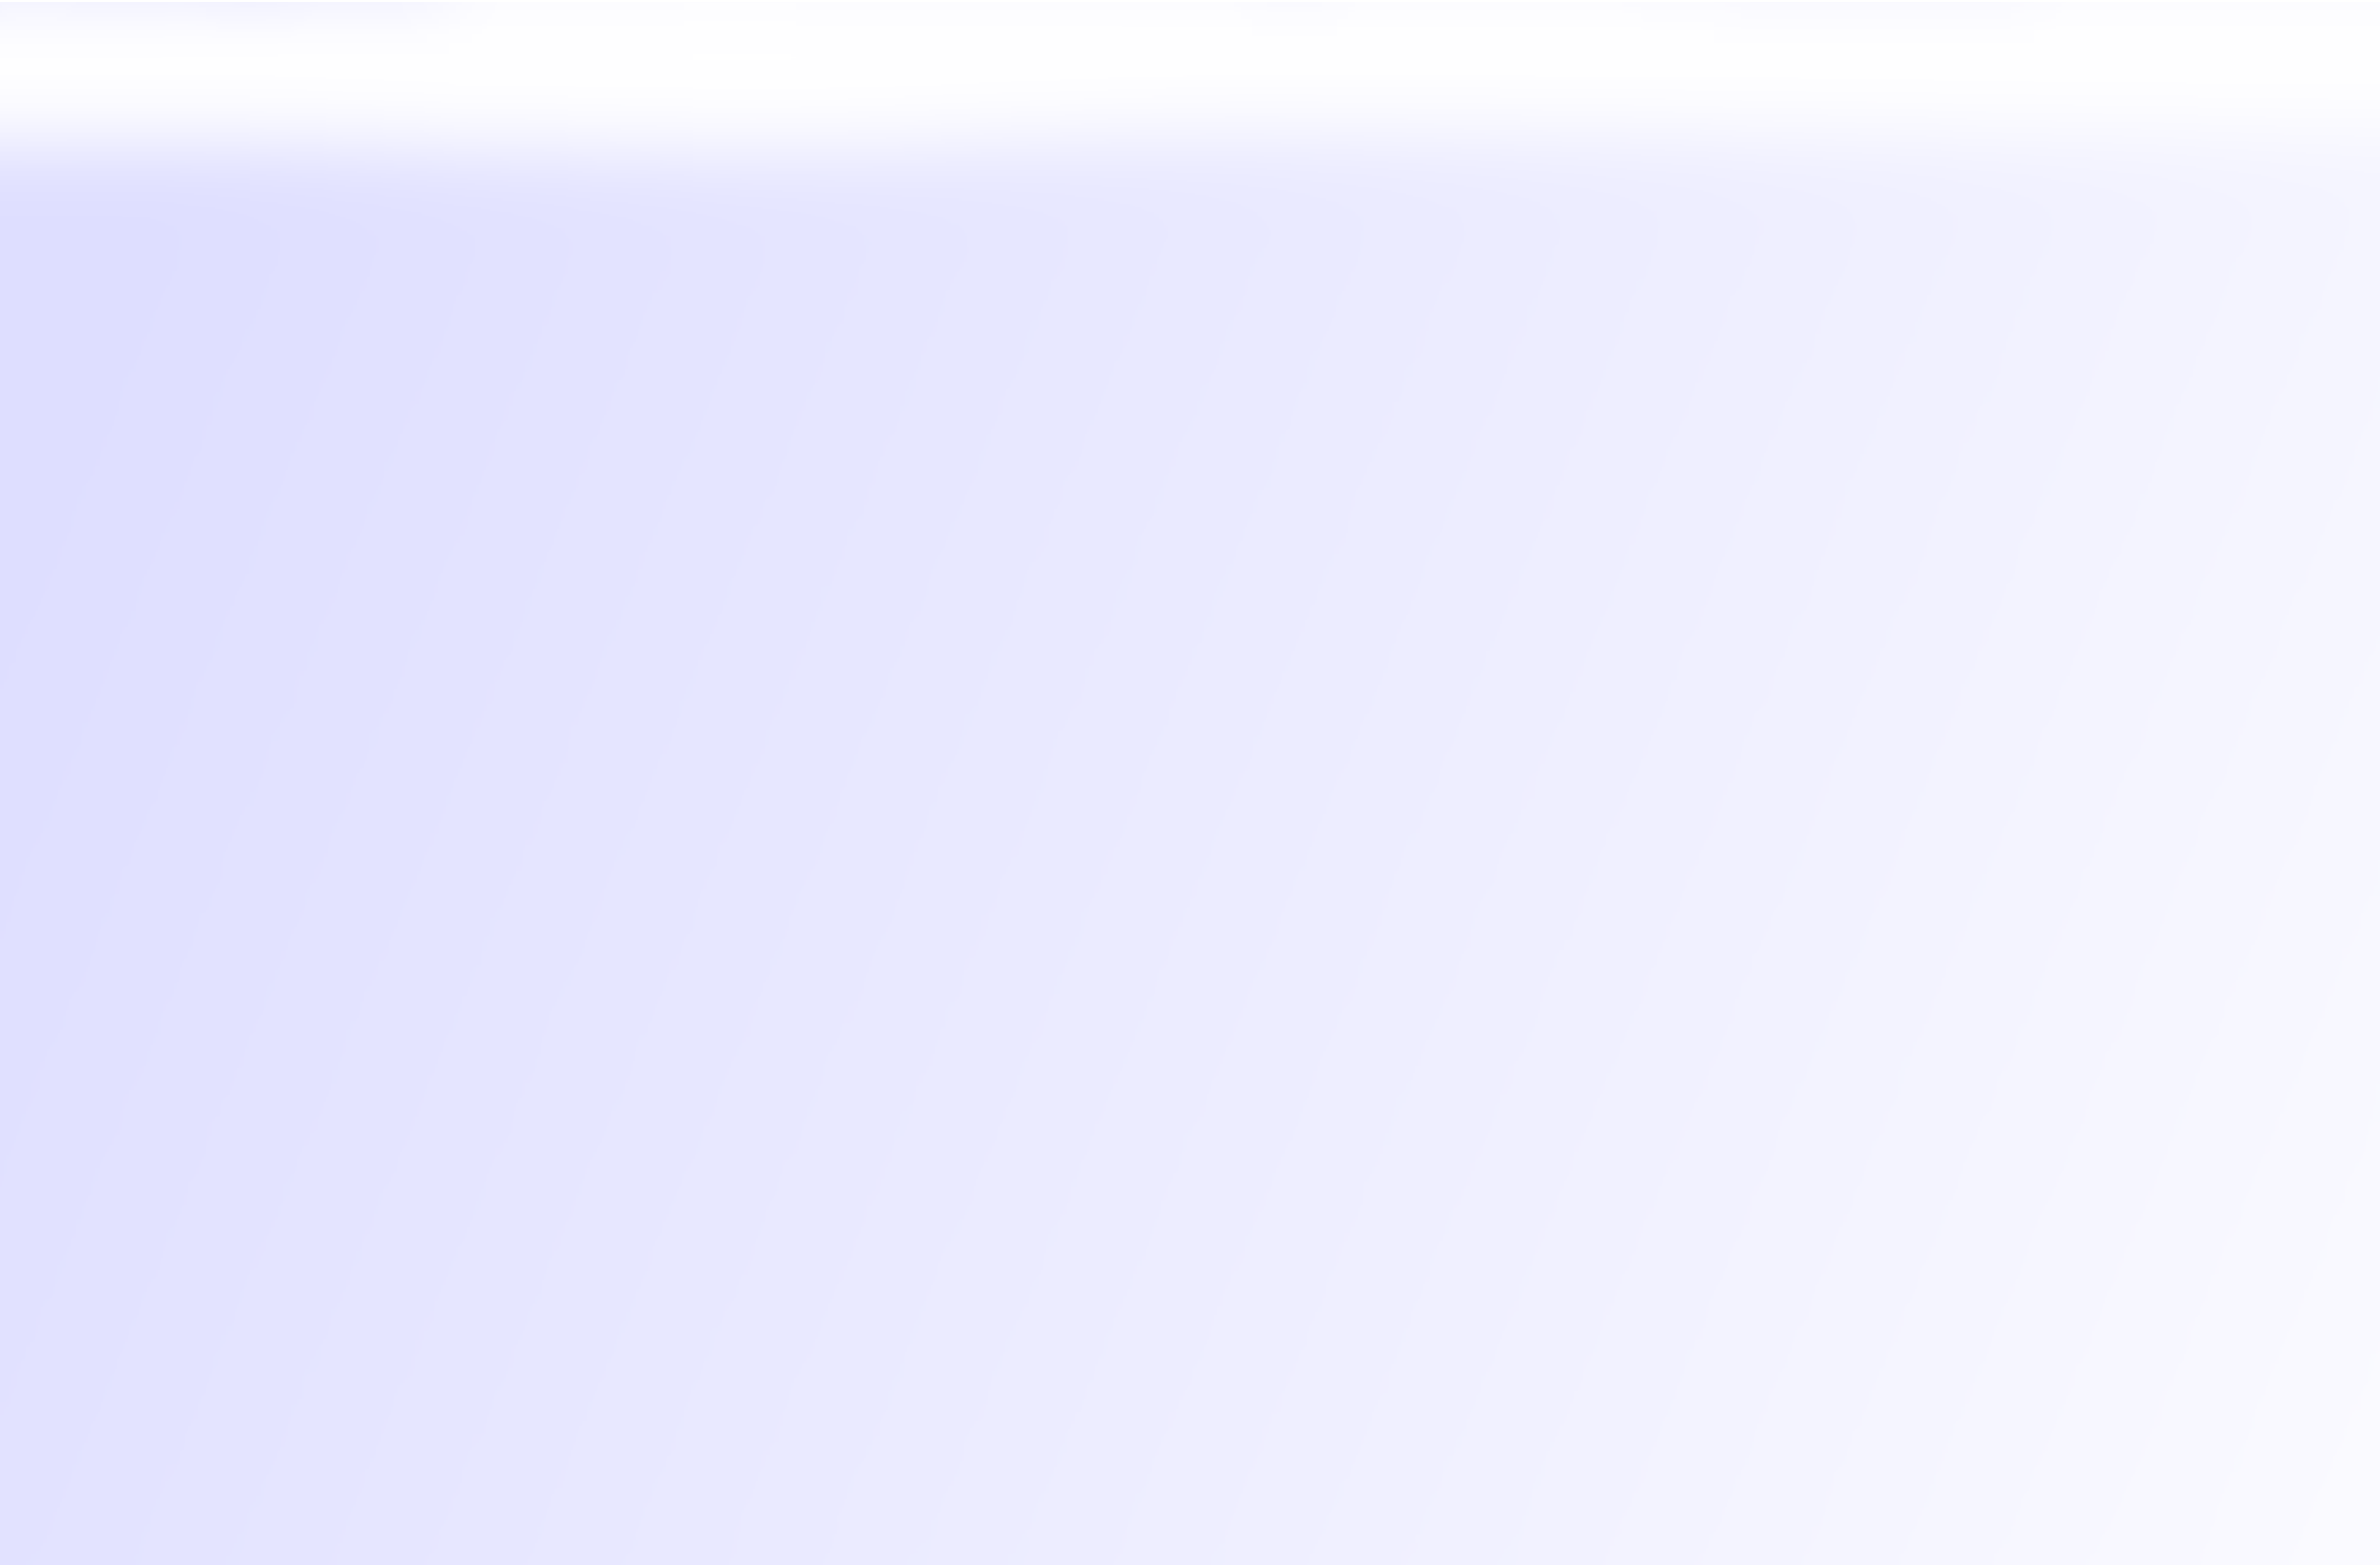
\includegraphics[height=1.1\textheight]{background}};
\end{tikzpicture}
}

\begin{poster}{
	grid=false,
	borderColor=bordercol, % Border color of content boxes
	headerColorOne=headercol1, % Background color for the header in the content boxes (left side)
	headerColorTwo=headercol2, % Background color for the header in the content boxes (right side)
	headerFontColor=headerfontcol, % Text color for the header text in the content boxes
	boxColorOne=boxcolor, % Background color for the content in the content boxes
	headershape=roundedright, % Specify the rounded corner in the content box headers
	headerfont=\Large\sf\bf, % Font modifiers for the text in the content box headers
	textborder=rectangle,
	background=user,
	headerborder=open, % Change to closed for a line under the content box headers
	boxshade=plain
} 
%
%----------------------------------------------------------------------------------------
%	TITLE AND AUTHOR NAME
%----------------------------------------------------------------------------------------
%
{
\includegraphics[scale=0.6]{uob-logo.eps}} % left logo
{\sf\bf\huge 
	Untangling the chromatin conformation \\ of the \textit{GNG12-AS1/DIRAS3} locus}
{\vspace{0.5em} \normalsize 
	Stephen Richer\textsuperscript{1} (\textcolor{blue}{\underline{s.richer@bath.ac.uk}}),
	Giuseppina Pisignano\textsuperscript{1}, 
	Stefan Schoenfelder\textsuperscript{2}, 
	\\ 
	Cameron Osborne\textsuperscript{3}, 
	Peter Fraser\textsuperscript{2}, 
	Dorothy Buck\textsuperscript{1}, 
	Adele Murrell\textsuperscript{1} \\ 
{\vspace{0.5em} 
	\textsuperscript{1}University of Bath, UK,
	\textsuperscript{2}Babraham Institute, Cambridge, UK,
	\textsuperscript{3}King's College London, UK}} 
{
\includegraphics[scale=0.13]{qrcode}} % right logo

%----------------------------------------------------------------------------------------
%	INTRODUCTION
%----------------------------------------------------------------------------------------

\headerbox{Introduction}{name=introduction,column=0, row=0}{

\begin{itemize}[leftmargin=*]
\item Here we study chromatin organisation at the imprinted \textit{GNG12-AS1/DIRAS3} locus.
\item This locus displays negative gene non-autonomy - \textit{GNG12-AS1} and \textit{DIRAS3} are reciprocally expressed - but the underlying mechanism remains unknown.
\item To investigate this we compare chromatin organisation between cell lines with contrasting epigenetic profiles.
\end{itemize}

\begin{center}
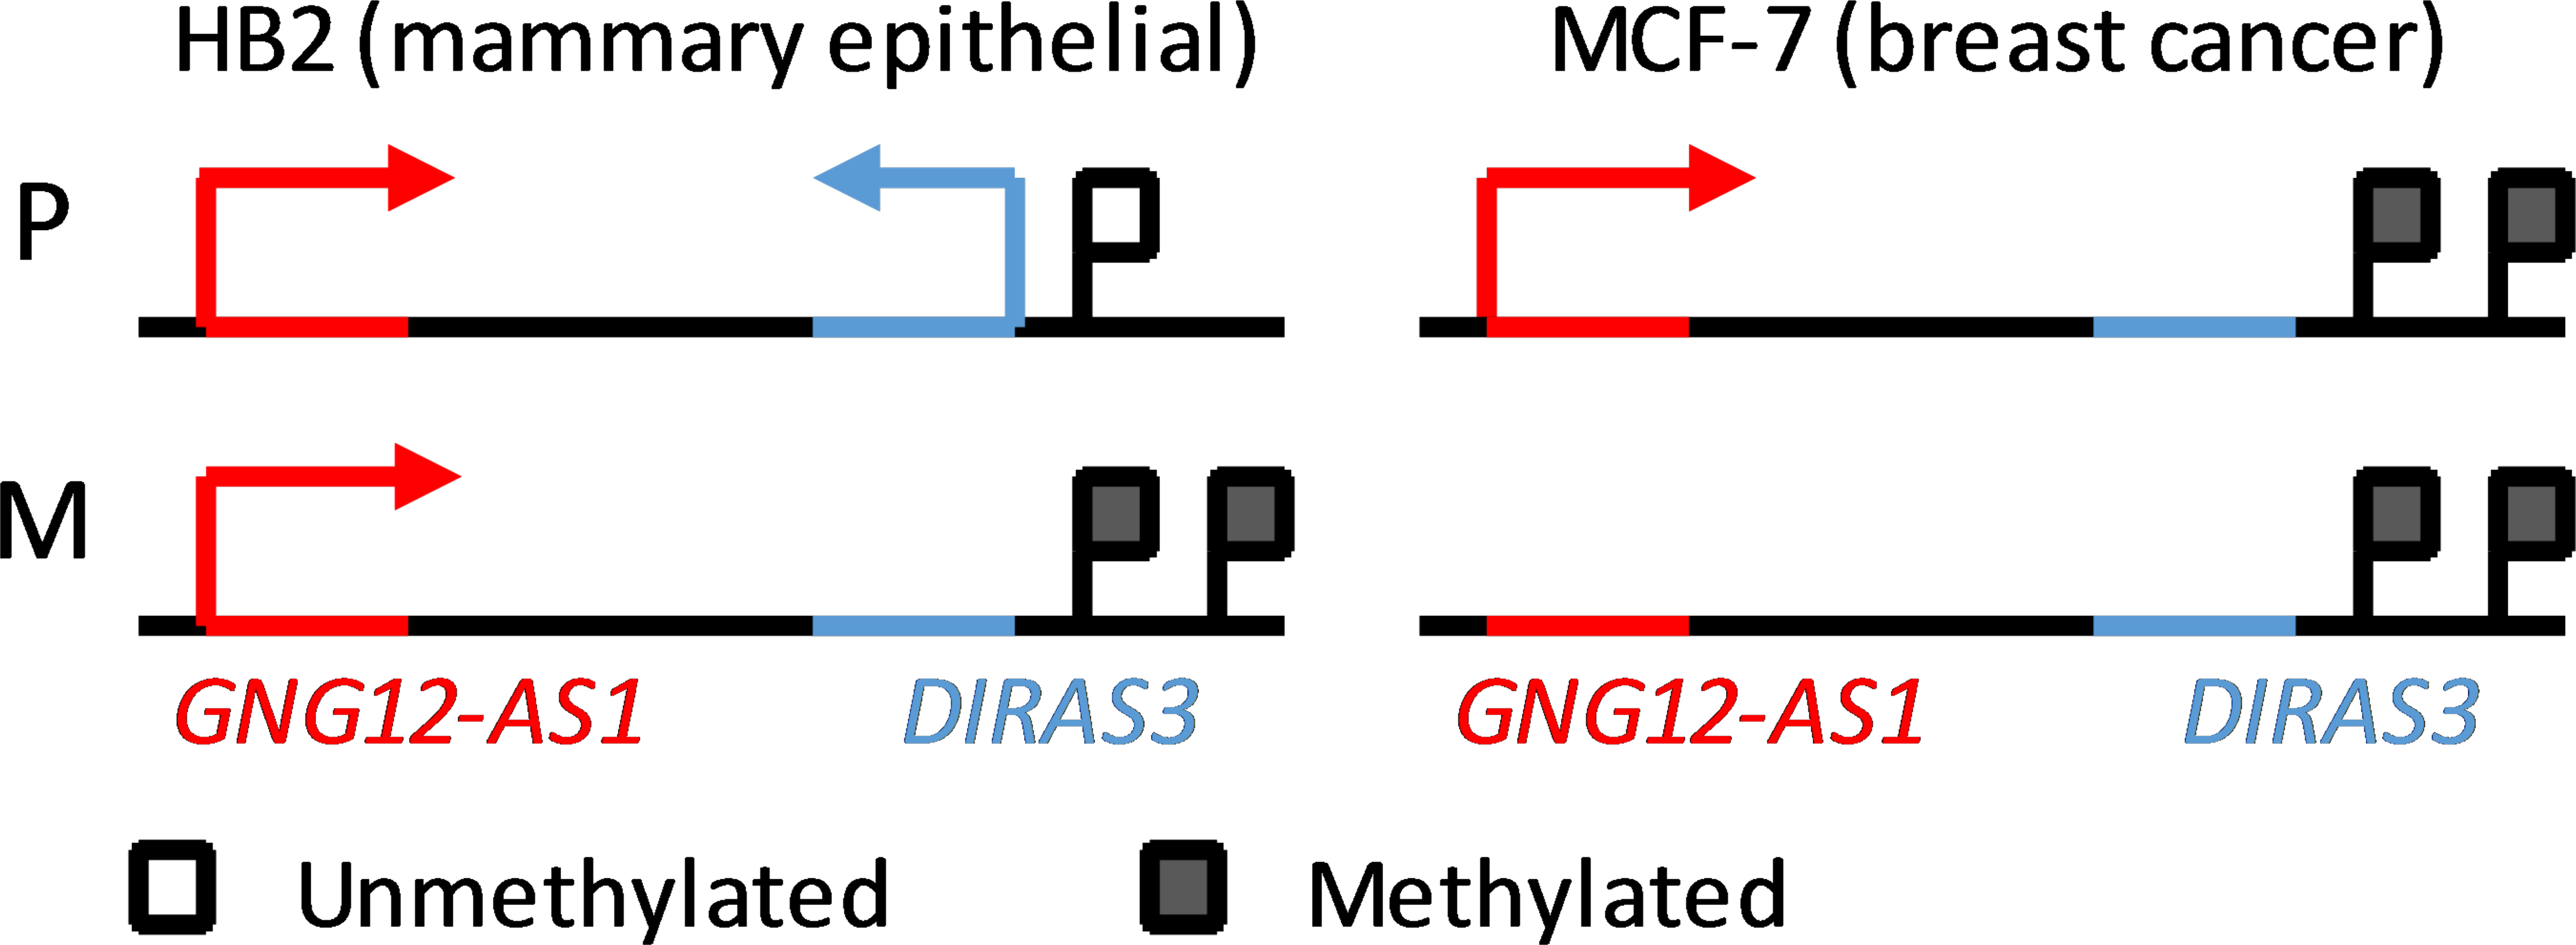
\includegraphics[width=1.0\linewidth]{mcf7_figure}
\captionof{figure}{Imprinted gene expression at the \textit{GNG12-AS1} locus in HB2 and MCF7 cell lines.}
%(chr1: 68,297,971 - 68,668,670)
\end{center} 
}

%----------------------------------------------------------------------------------------
%	MATERIALS AND METHODS
%----------------------------------------------------------------------------------------

\headerbox{Materials and Methods}{name=methods,column=0,below=introduction}{

\begin{description}
\item[Capture HiC] Generate high-resolution chromatin conformation maps of the \textit{GNG12-AS1} locus in HB2 (mammary epithelial) and MCF7 (breast cancer) cell lines.
\item[Bioinformatics] Compare TAD structure and assess changes in contact frequency between cancer and non-cancer cell lines.
\end{description}

\begin{center}
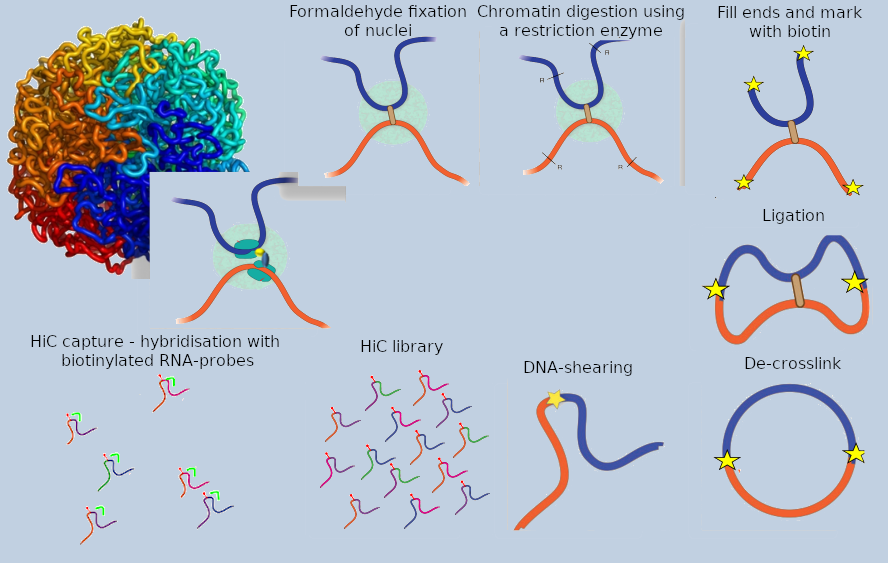
\includegraphics[width=1.0\linewidth]{hic_technique}
\captionof{figure}{Overview of capture HiC protocol.}
\end{center}

}

%----------------------------------------------------------------------------------------
%	CONCLUSION
%----------------------------------------------------------------------------------------

\headerbox{Future work}{name=conclusion,column=0,below=methods}{

\begin{itemize}[leftmargin=*]
\item Create 3D visualisation of DNA looping based on HiC interaction map.
\item What are biological implications of reduction in interaction frequency, between HB2  and MCF7, at \textit{GNG12-AS1} locus?
\item Investigate unexpected changes up-down and down-stream of \textit{GNG12-AS1} locus.
\item Allele specific HiC to study effect of imprinting on chromatin organisation. 
\item Refine methods to robustly compare TAD changes between samples.
\end{itemize}

}

%----------------------------------------------------------------------------------------
%	REFERENCES
%----------------------------------------------------------------------------------------

\headerbox{References}{name=references,column=0,
	below = conclusion, above = bottom}{

\smaller % Reduce the font size in this block
\renewcommand{\section}[2]{\vskip 0.05em} % Get rid of the default "References" section title
\nocite{*} % Insert publications even if they are not cited in the poster

\bibliographystyle{unsrt}
\bibliography{poster-abr} 
}

%----------------------------------------------------------------------------------------
%	RESULTS 1
%----------------------------------------------------------------------------------------

% To reduce this block to 1 column width, remove 'span=2'
\headerbox{Chromatin organisation at \textit{GNG12-AS1}} {
	name = results1, span = 2, column = 1}{ 
%------------------------------------------------
\begin{center}
\includegraphics[width=1.0\linewidth]{GNG12_AS1_DIRAS3_ontad_sum_3000_count}
\captionof{figure}{
HiC interaction map\textsuperscript{\cite{Ramirez2018}}, summed across 2 replicates, for HB2 (top) and MCF7 (bottom).
}
\end{center}
%------------------------------------------------

\begin{itemize}[leftmargin=*]
\item TAD boundaries\textsuperscript{\cite{An2019}} align well with CTCF sites and reveal a complex hierarchical structure.
\item These structures likely represent a consensus set of domains that exist among the cell population and across the cell cycle.
\item However, there is some inconsistency in TADs between replicates.
\end{itemize}

}

%----------------------------------------------------------------------------------------
%	RESULTS 2
%----------------------------------------------------------------------------------------
% To reduce this block to 1 column width, remove 'span=2'
\headerbox{Chromatin conformation changes between HB2 and MCF7} {
	name = results2, span=2, column = 1, 
	below = results1, above = bottom}{
%------------------------------------------------

\begin{center}
\includegraphics[width=1.0\linewidth]{GNG12_AS1_DIRAS3_HB2_WT_vs_MCF7-logFC}
\captionof{figure}{
Log\textsubscript{2} FC of MCF7 over HB2 with differential interactions\textsuperscript{\cite{Lun2015}}. \textcolor{red}{Red} = increase in MCF7.
}
\end{center}

\begin{itemize}[leftmargin=*]
\item Broad regions of reduced contact frequency, in MCF7, were detected approximately 1.5 megabases downstream of \textcolor{orange}{\textit{\textbf{GNG12-AS1}}}, near \textcolor{red}{\textit{\textbf{PDE4B}}}, \textcolor{black}{\textit{\textbf{MIRE1}}} and \textcolor{yellow}{\textit{\textbf{SGI1P}}}.
\item Increases in contact frequency, in MCF7, were also detected between \textcolor{green}{\textit{\textbf{LRRC7}}} and a number of regions approximately 500 kilobases upstream of \textcolor{orange}{\textit{\textbf{GNG12-AS1}}}.
\end{itemize}
}

\end{poster}

\end{document}